\subsection{Front End}
We are using wordpress \cite{word} for front end design. We created a website on which it displays all the live tests student can attempt and submit. We are using Ninja plugin in wordpress for creating tests online and publishing the same. The test must have a roll number field which will be used to identify the student. For now any student visiting the website can attempt any of the displayed live tests. About setting the test, Admin is the only teacher yet which can set test and publish it online on website. \\
\begin{figure}[H]
    \centering
    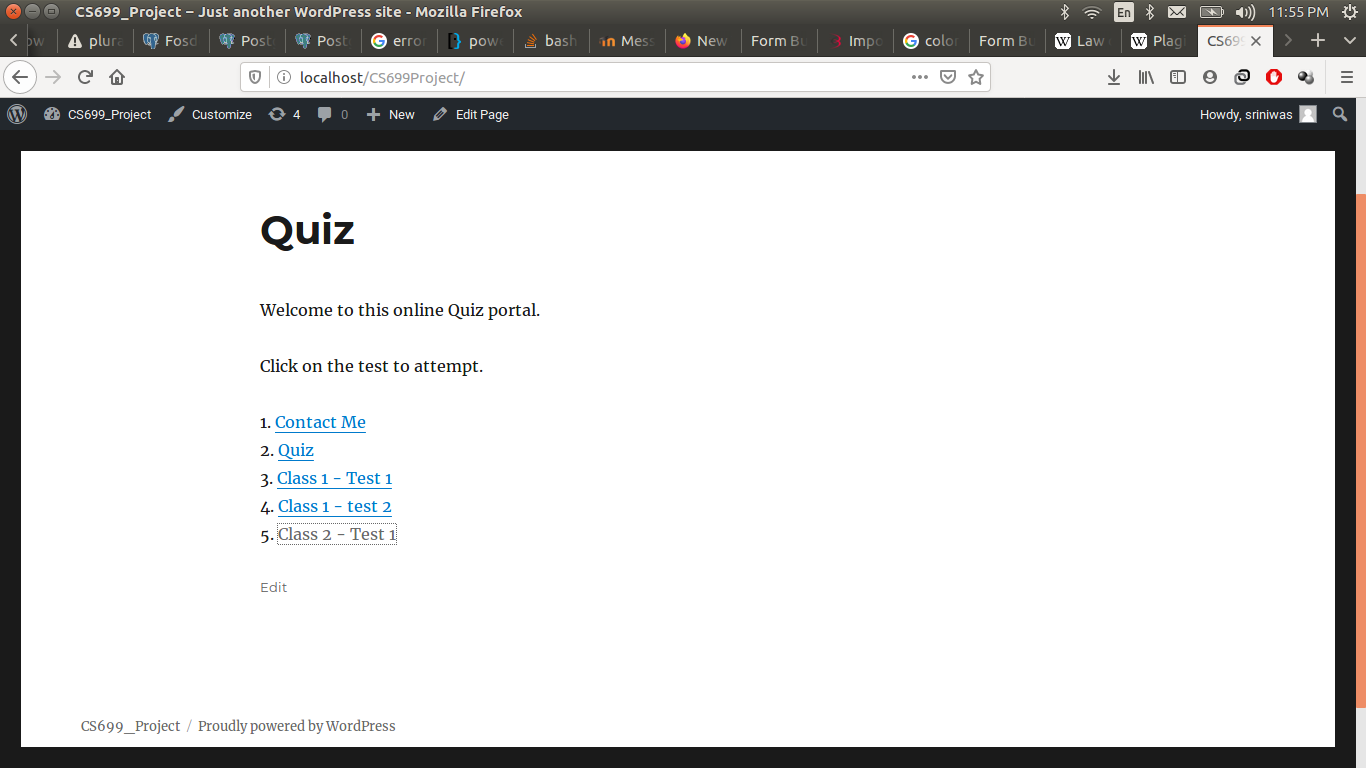
\includegraphics[width=0.5\paperwidth]{images/Website.png}
    \caption{A small overlook of the website}
    \label{fig:galaxy}
\end{figure}

Here are some tests we have already published for testing and analysis purpose. Students can attempt to submit responses for these tests. The asterisk mark fields are mandatory to fill, otherwise form will not get submitted.
\begin{figure}[H]
\label{fig1}
      \centering
  \begin{minipage}[b]{0.45\textwidth}
    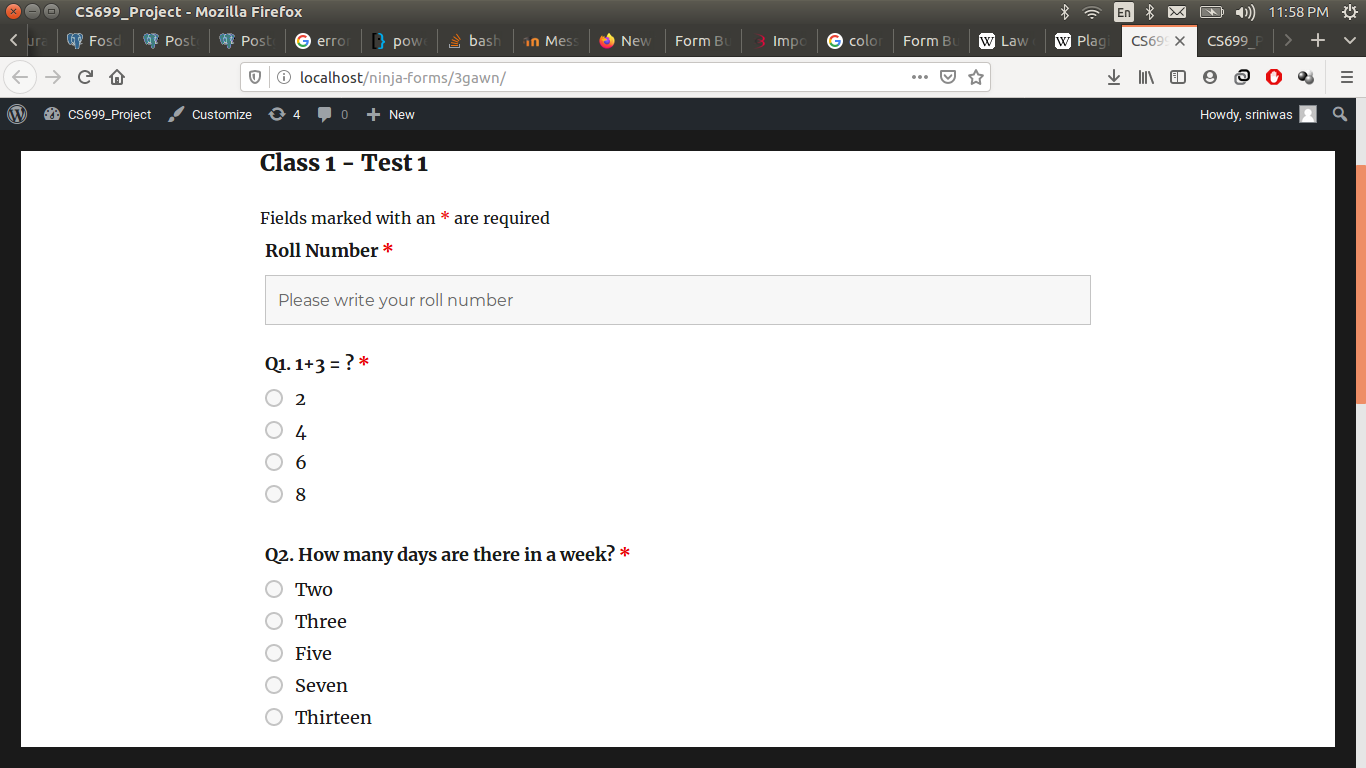
\includegraphics[width=\textwidth]{images/Test11.png}
    \caption{Demo Test1 Page 1}
  \end{minipage}
  \hfill
  \begin{minipage}[b]{0.45\textwidth}
    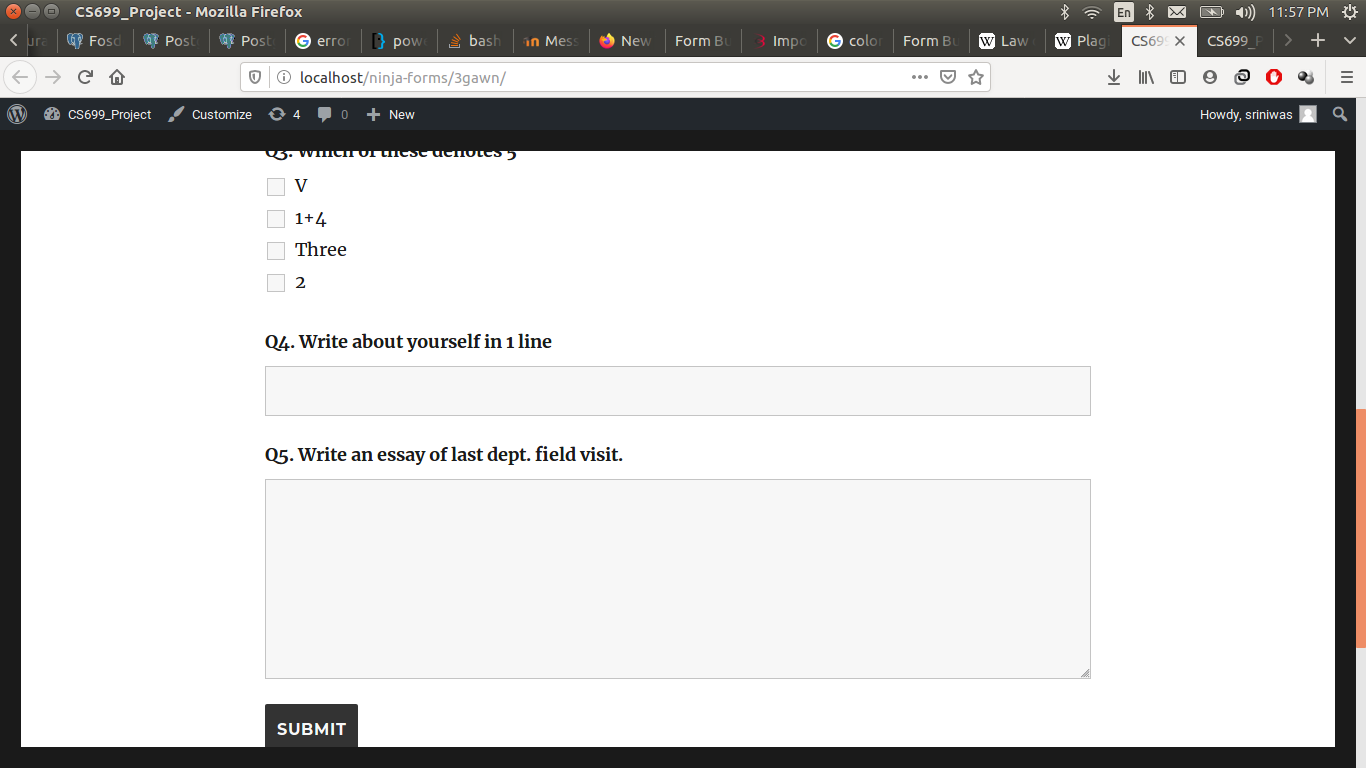
\includegraphics[width=\textwidth]{images/Test12.png}
    \caption{Demo Test1 Page 2}
  \end{minipage}
  \hfill
\end{figure} 
Every test must contain a field for roll number which will be used to detect uniquely pairwise plagiarism index among the submitted responses. Here is another example of a test.
\begin{figure}[H]
\label{fig1}
      \centering
  \begin{minipage}[b]{0.45\textwidth}
    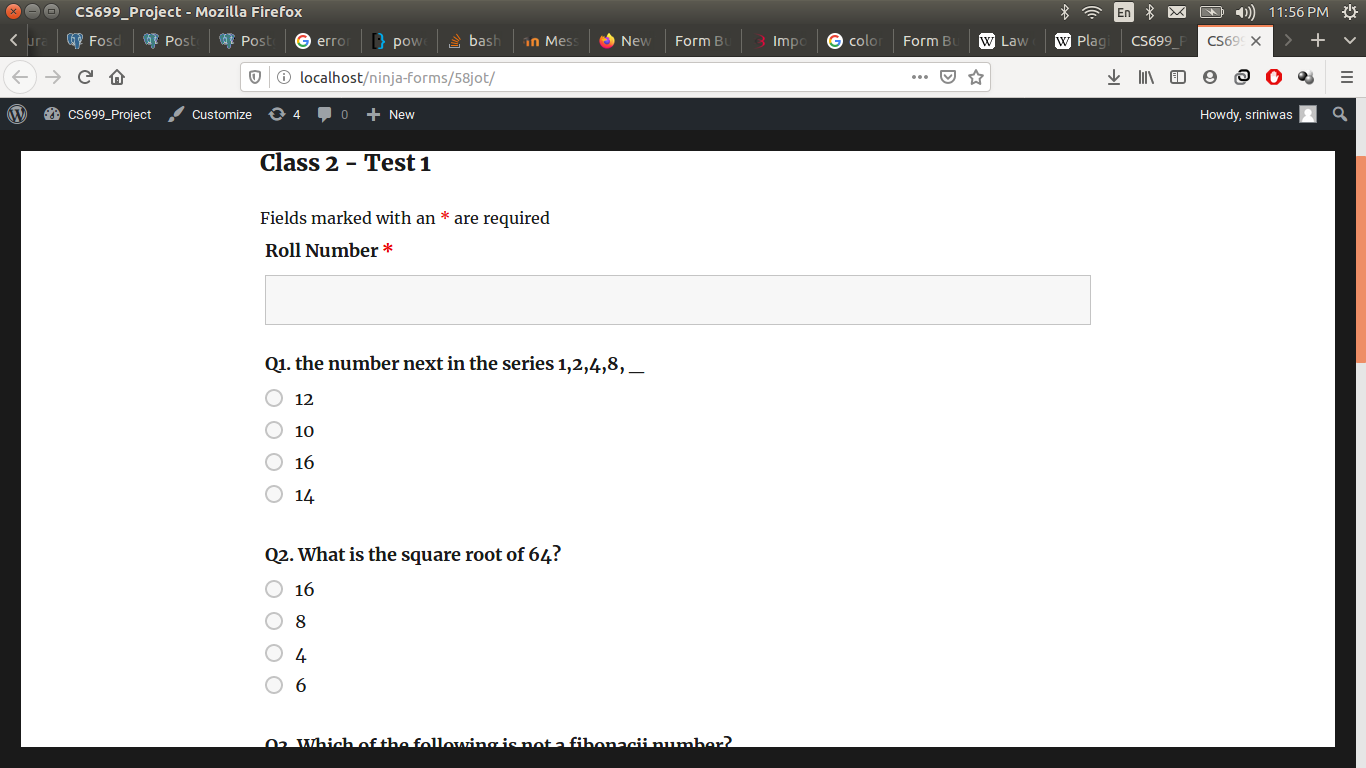
\includegraphics[width=\textwidth]{images/Test2.png}
    \caption{Demo Test2 Page 1}
  \end{minipage}
  \hfill
  \begin{minipage}[b]{0.45\textwidth}
    \includegraphics[width=\textwidth]{images/Test21.png}
    \caption{Demo Test2 Page 2}
  \end{minipage}
  \hfill
\end{figure} 
Admin can create new test using the provided interface. We are using Ninja forms plugin in wordpress for this purpose. Teacher can add any number of questions of any type in any order. And he will have to provide solutions in a csv file of the corresponding test. This is strongly required for the plagiarism detection model of ours. 
\begin{figure}[H]
    \centering
    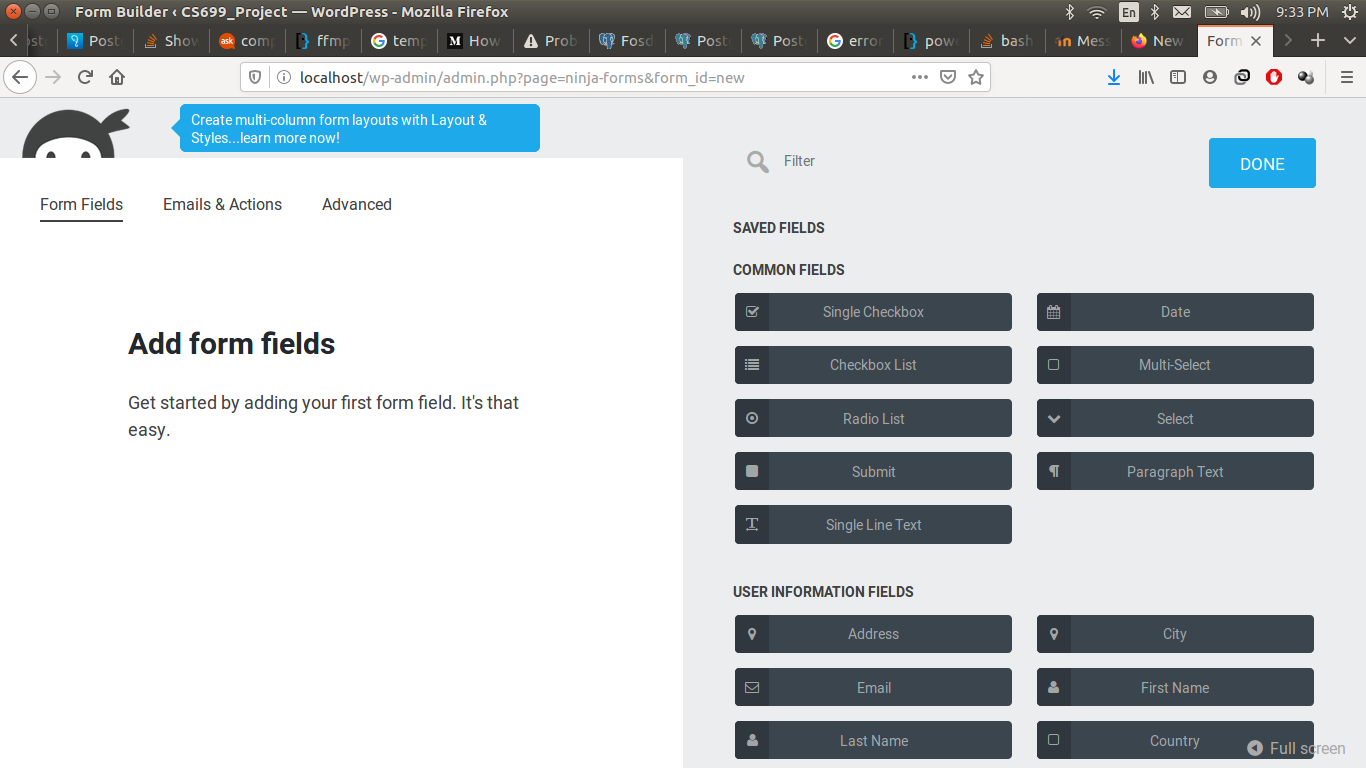
\includegraphics[width=0.5\paperwidth]{images/test_form.png}
    \caption{Sample blank form for test creation}
    \label{fig:galaxy}
\end{figure}
When deadline for attempting test is over, admin will disable the link of that test. Now after getting all the submissions/responses, while evaluating teacher will be provided with the option of applying plagiarism check or not. Also if one chooses to apply the plagiarism check while evaluating the responses, he can also customise the weights given to different algorithms according to the requirements of the test. \\
Eventually, teacher will be provided with a csv file which will have plagiarism indices in descending order for all pairs of responses. He can set a threshold passing which will mean the student has not cheated in the test.
\begin{figure}[H]
\label{fig1}
      \centering
  \begin{minipage}[b]{0.45\textwidth}
    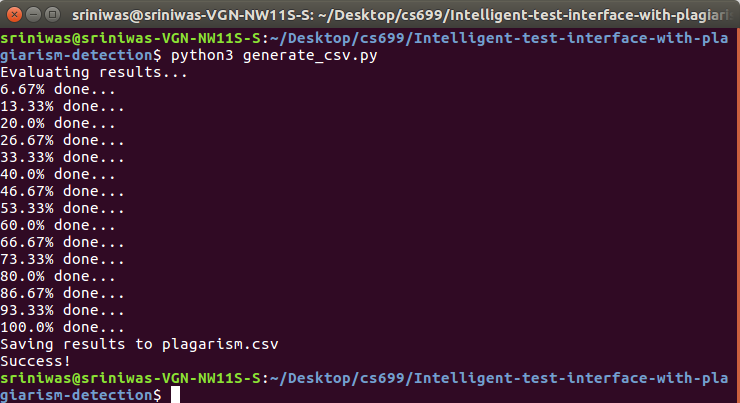
\includegraphics[width=\textwidth]{images/python_script.png}
    \caption{Running python script to evaluate plagiarism index}
  \end{minipage}
  \hfill
  \begin{minipage}[b]{0.45\textwidth}
    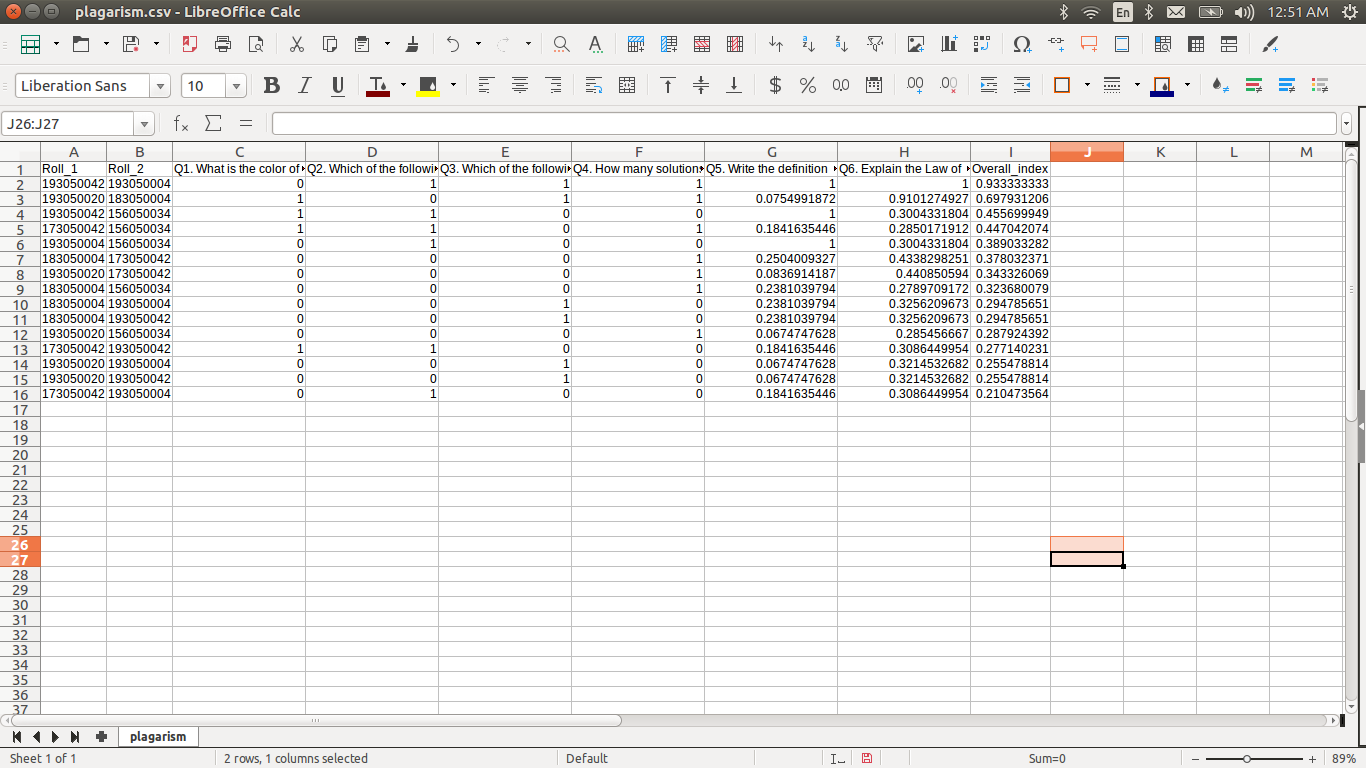
\includegraphics[width=\textwidth]{images/results_csv.png}
    \caption{CSV file consisting of plagiarism indices}
  \end{minipage}
  \hfill
\end{figure} 
If n responses are submitted in total the csv file having final result of plagiarism indices will have $\binom{N}{k}$ entries in it in sorted order(highest plagiarised index to lowest plagiarised index).

\subsection{Back End}
 A test can have briefly have two sort of questions :
 \begin{enumerate}
     \item Subjective Type (Single Line or Multiple Line)
     \item Objective Type (MCQs with single choice or multiple choice)
 \end{enumerate}
 To apply plagiarism test on subjective type questions we are using various string matching algorithms. One of the popular n-gram based similarity algorithm cosine similarity works on vectors of frequency of letters. Since results from this algorithm was significantly accurate, we modified cosine similarity for word frequency vectors and it is giving even better results. So to get best results of plagiarism indices, teacher should give this algorithm a significant weight. \\ \\
 \textbf{Weights csv file : } This file consists of weights corresponding to the algorithms Least Common Subsequence (LCS), Cosine Angle, Cosine Angle (words) and Jacard Index.
 Admin can modify these weights according to the requirements of his test. According to the weights given in this csv, the Subjective questions' plagiarism index will get evaluated. \\ \\
 \textbf{Solution csv file :} For each test teacher is supposed to provide a csv consisting of correct solutions. This csv file is useful while evaluaing the plagiarism index for MCQs. If two students have selected the same option/options then there could be two possible cases : First is that both have marked correct answer, then the chances are low that they have copied so we are giving index 0 to such a case. \\
 Second case is that both have marked same wrong option/options, here chances are comparatively high that they have copied (even higher in case of multiple choice MCQs), so we are giving index 1 to these sort of matches. Since MCQs themselves have low weightage of overall marks, in case it was just an coincidence that incorrect answers matched then also it won't effect the plagiarism index adversely until Subjective Questions of these two also caught to have some plagiarism index. \\
 
 Solution csv provided by teacher should also contain the marks distribution for the questions. After we are done evaluating individual question's plagiarism index, at the end these indices will be given weights in the ratio of their distribution of marks in the test. The outcome from this will be our final and fair Plagiarism index between those two students. 
 
 
 

